\scanpage{86}
UNIVERSITE DES SCIENCES\\
ET TECHNIQUES DU LANGUEDOC

\figure{\begin{tikzpicture}\draw[dashed] (0,0)--(2,0);\end{tikzpicture}}

Service de la Scolarité\\
AMC/GJ

Montpellier, le 17 Juillet 1975

\uline{Diffusion :} Liste H\\
N°4617

AVIS DE SOUTENANCE\\
D'UNE THESE DE DOCTORAT D'ETAT

\figure{\begin{tikzpicture}\draw (0,0)--(2.4,0);\end{tikzpicture}}

\uline{Nom et prénom du candidat} : FOLLET Michel

\uline{Titre de la Thèse} : Etude physicochimique de la réactivité du cycle triazine : Synthèse et analyse spectrale de dérivés bicycliques.

\uline{Date, heure et lieu de soutenance prévus} :\\
8 Septembre 1975 à 17 Heures,\\
Salle de cours n° 9.

\uline{Nom du Directeur de thèse} : Professeur JACQUIER.

\uline{Désignation du laboratoire où la thèse est préparée} : Laboratoire de Synthèse et d'Etude Physicochimique d'Hétérocycles Azotés.

\uline{Résumé de la thèse} : Ce travail porte sur la série de la triazine - 1,2,4 , plus particulièrement sur les dérivés de l'acide thioxo-3 oxo-5 tétrahydro-2,3,4,5 triazine carboxylique -6. Différentes méthodes de synthèse de triazolo-triazines et triazolyl - triazines sont données. L'analyse spectrale de ces composés est faite par UV, RMN et spectrométrie de masse.

\uline{Durée approximative des recherches ayant abouti à la thèse} : 4 ans.

\uline{Noms des rapporteurs} :

JACQUIER R., Professeur, Chimie organique, U.S.T.L.\\
GRANGER R., Professeur, Chimie organique; Université MONTPELLIER I.\\
VIALLEFONT Ph. Professeur, Chimie organique, U.S.T.L.

\uline{Composition du jury} :

JACQUIER R., Professeur, Chimie organique, U.S.T.L. (Président)

GRANGER R., Professeur, Chimie organique, Université MONTPELLIER I (Membre extérieur choisi en raison de sa compétence scientifique)

DESCHAMPS J. Professeur, Chimie-physique, Faculté de Pau et des Pays de l'Adour (Membre étranger à la spécialité du candidat)

VIALLEFONT Ph. Professeur, Chimie organique, U.S.T.L.

DAUNIS J., Chargé de Recherche CNRS, Chimie organique, U.S.T.L.

LE SECRETAIRE GENERAL

\figure{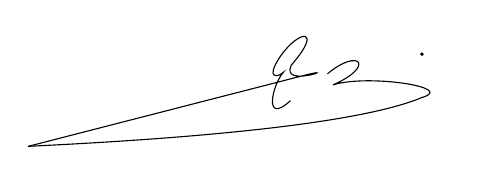
\begin{tikzpicture}[x=1cm,y=1cm]
\draw (0,0)--(3.5,.9) .. controls (4,1.03) and (3.2,.73) .. (3.34,1.03)
.. controls (3.75,1.5) and (3.45,1.5) .. (3.2,1.14)
.. controls (3,.84) and (3.18,.88) .. (3.24,.94)
.. controls (3.1,.78) and (2.98,.26) .. (3.33,.58);
\draw (3.8,.92) .. controls (4.2,1.26) and (4.42,1.02) .. (3.87,.78)
.. controls (4.3,.92) and (5.45,.75) .. (5,.62)
.. controls (4,.2) and (1,.05) .. (0,0);
\fill (5,1.17) circle (.025);
\end{tikzpicture}}

\uline{E. SIAU}

MR LE PROFESSEUR GROTHENDIECK A.\\
MATHEMATIQUES\hfill 5-856

\margin{85}
